\chapter{Useful Figures and Formulas in Chemistry}
\textbf{The periodic table of the elements} is arguably one, if not, the most important thing to have when learning chemistry. For the high school level, the most useful periodic table is the one that has ion charges of the elements.

\textbf{A table of common symbols used in formulas} can be found in table \ref{tab:c0}
\begin{table}
    \centering
    \begin{tabular}{|c|c|c|c|} \hline 
         Symbol&  Name&  Unit& Explanation\\ \hline 
         n& Number of moles& mol& \ref{sec:c-mole}\\ \hline 
         m& Mass& g& \\ \hline 
         M& Molarity& g/mol& \ref{sec:c-mole}\\ \hline 
         V& Volume& L& \\ \hline 
         \%A& Percentage composition of element \ch{A}& \%& \ref{sec:c-composition}\\ \hline 
         D& Density& g/l& \\ \hline
    \end{tabular}
    \caption{A table of common symbols used in formulas}
    \label{tab:c0}
\end{table}

\section{Formulas}
In this section, each name will followed by a reference to the equation (or the section) that explains the formula. There are no units included for the sake of memorization but you should always keep the unit in the back of your head, or better yet, remember the conversion factor procedure.

\textbf{Number of moles} when given mass and molar mass (\ref{eq:c-mol}):
\begin{equation} n = \frac{m}{M} \end{equation}

\textbf{Number of moles of a gas in standard condition} (\ref{eq:c-mol-in-gas}):
\begin{equation} n = \frac{V}{22.4} \end{equation}

\textbf{Percentage composition} (\ref{eq:c-percentage-composition}):
\begin{equation}
    A\% = \frac{m_A}{m_{AB}}\times100\%
\end{equation}

\chapter{Stoichiometry}
Stoichiometry simply means that we are dealing with chemical reactions and the quantitative data from such reactions (like weight, volume, number of atoms, etc...).

\section{The mole — the central number of chemistry}\label{sec:c-mole}
How many items are there in a triplet? $3$. How much is a dozen? $12$. Now we have a new definition:
\begin{equation}
    \text{A mole} = 6.02\times10^{23}
\end{equation}
Similar to how half a dozen is $0.5\times12=6$, you can tell other scientists that you have a certain number of moles of \textit{something}. Note that a mole is still a quantity and not a unit — you have a mole of something. As a conversion factor, a mole is:
\begin{equation}
    \frac{1\text{mol of item}}{6.02\times10^{23}\text{ items}}
\end{equation}

A mole of atoms of an element acts as the central unit to convert between different units or elements in a reaction.

\textbf{Molar mass} is the mass of $1$ mole of an element while the \textbf{formula mass} of a compound is the sum of all atoms in that compound. They are both similar in value but different in the unit: molar mass's unit is usually in grams per mole while formula mass is in the atomic unit, which is $1/12$ the weight of a carbon atom (or about $1$ hydrogen atom). The atomic unit will be abbreviated as "u" throughout this note.

\textbf{To calculate the number of moles}, you can see how many times the molar mass you have of the element \ch{A}:
\begin{equation}
    \label{eq:c-mol}
    n = \frac{m\text{ g}}{M\text{ g/mol}}
\end{equation}

$1$ mole of any gas at \textbf{standard temperature and pressure} or \textbf{STP} occupies exactly $22.4$ litres. That property only appears for gasses but not liquids or solids. If you want to calculate \textbf{the number of moles in a volume of gas}:
\begin{equation}
    \label{eq:c-mol-in-gas}
    n = V\text{ L} \times \frac{1\text{mol}}{22.4\text{L}}
\end{equation}

\textbf{Molarity} is the number of moles of the chemical per litre of a solution. It indicates how many moles of the chemical are presented in a litre of a solution — similar to density but in this case, it is the number of atoms over 1 litre of the solutions. Because a solution will include both the chemical and the water, the actual amount of water present in the solution is not $1$ litre — you add water \textit{up to} $1$L, NOT $1$L \textit{of water}.

\textbf{The relationship between a mole and the chemical formula} is in the proportion. For example, the element dihydrogen monoxide\footnote{Normal people usually called it "water"} has the formula \ch{H2O}, which states that for every oxygen atom, there are two hydrogen atoms. If you now have a mole of oxygen, you need to double that amount to have two moles of hydrogen in your compound.

\section{Composition analysis}\label{sec:c-composition}
Before calculating anything, it is usually appropriate to know the chemicals you are using. The first thing to realize is that not all atoms are similar in weight; consider a composition of \ch{H2} and \ch{O}, the \ch{O} will make up most of the mass in a molecule — this happened because one \ch{O} elements weight $16$u while a hydrogen atom weights at about $1$u.

An example to determine the \textbf{percentage composition} or how much each element takes up the total mass in a water molecule: first calculate how much each element weights in the entire compound:
\[
    1\text{g H/mol H}\times2=2\text{g H/mol H}_2\text{O}
    \qquad
    16\text{g O/mol O}\times1=16\text{g O/mol H}_2\text{O}
\]
In this stage, we calculate the weight of individual items that make up our compound. From the formula to create $1$ mole of water, you will need two moles of hydrogen and $1$ mole of oxygen — this is proportional to having 2 atoms of hydrogen and 1 atom of oxygen. Honestly, you could just make this calculation using atomic units instead of grams and it would work about fine but for the sake of accuracy, please refrain from doing so. Anyway. we will now total up the weight of individual elements to get the weight of the entire compound before calculating the percentage:
\[
    2 + 16 = 18\text{g H}_2\text{O/mol H}_2\text{O}
\]
\[
    \%\text{H}
    = \frac{2 \text{g H}}{18 \text{g H}_2\text{O}}\times100
    = 11\%\text{H}
\]
Despite you need two atoms of hydrogen to build a single molecule, clearly that single hydrogen atom takes up more weight.

The general formula to calculate the \textbf{percentage composition} with the mass of an element $m_A$ and the compound's mass $m_{AB}=m_A+m_B$ is:
\begin{equation}
    \label{eq:c-percentage-composition}
    \%A = \frac{m_A}{m_{AB}}\times100\%
\end{equation}

To calculate an \textbf{empirical formula}, we start by pretending we have $100$g of the substance: $11$g of that substance would be hydrogen and $89$g would be oxygen. We now divide each of those numbers by the molar mass to obtain the number of moles in that mass:
\[
    11\cancel{\text{g H}}
    \frac{1\text{mol H}}{1\cancel{\text{g H}}}
    = 11\text{mol H}
    \qquad
    89\cancel{\text{g O}}
    \frac{1\text{mol O}}{16\cancel{\text{g O}}}
    = 5.5625\text{mol O}
\]
Then divide them by the smallest factor (in this case $5.5625$) to get the ratio between elements:
\[ 11/5.5625=1.977 \]
Because of the estimations in our equation, it is appropriate to assume that it is 2 moles of hydrogen for every oxygen atom or \ch{H2O}.

If you were to simplify the process of calculating \textbf{empirical formula} into an equation, define the formula \ch{A_xB_y} and $n_A$ is the molar mass of \ch{A}, we have the ratio:
\begin{equation}
    x:y
    = \frac{\%A}{n_A} : \frac{\%B}{n_B}
    = m_A : m_B
\end{equation}

\section{Chemical equations}
A chemical equation usually indicates the proportion of the chemicals that participate in a reaction, essentially showing the mole of particles you need. 

\chapter{Electron Configuration}
\section{Introduction: The modern model of atoms}
This section is for a simplified explanation of what is going on. It is not required if you are in a hurry but is highly recommended to grasp the deeper understanding of the explanations in the latter sections.

Most of us are used to the fact that an electron flies around the nucleus in a fixed orbit. This is unfortunately an oversimplification of what happened but for a good reason. Throughout this chapter's model, an electron can move freely around a region rather than flying in a predetermined orbit. Every time you "observe" an electron, you take a picture of it which shows its position in space. As you take more pictures, you will eventually see where it is most likely to appear, and that is how you establish the orbit\footnote{In this case, we still call it an "orbit" but understand that it is a "region" in space where the electron has 90\% chance of appearing in it.} of the electron.

The first four atomic orbital shapes that you will see are s, p, d, and f. For larger atoms, there will be more electrons which require more space to be in, which will create more diverse region's shape (likewise, the outer shell in the classic atom model has more electrons than the inner shell). Each atomic orbital can store up to 2 electrons and will be filled from the smallest orbital to the biggest orbital (which will be called a "shell"). Lastly, the electrons are shy and they would love to occupy an orbital to themselves if possible using Hund's rule.

Of course, what is being said is still a simplification but it is enough for you to grasp the idea of what we are doing in this chapter. Particularly, the given model does not address the wave-particle duality of quantum mechanics nor the complexity of electron orbit; for your information, all of that is stepping on the line between physics and chemistry. Now, this section is the general analogy for you to understand but the latter sections will have a more academic approach to the topic for you to take tests.

\section{Quantum numbers}
There are three unique quantum numbers to describe an atomic orbital; this can be extended to describe an electron using the orbital it is in and its spin (the fourth quantum number). \textbf{The Pauli exclusion principle} says that each orbital only has 2 electrons with a different spin, which means that the four quantum numbers are essentially the ID of an electron.

\textbf{The principal quantum number ($n$)} indicates the relative size of the atomic orbital. This is relative to the "shell" of the electron in the classic atom model, so as the number of shells increases, there will be more electrons which leads to more atomic orbital. \textit{Most of the time}, a higher $n$ means that the orbital has higher energy and the electron will spend more time farther from the nucleus.
\begin{equation}
    n\in\mathbb{N}\setminus\{0\}
    \qquad 0 \leq n
\end{equation}

\textbf{The azimuthal quantum number\footnote{Also known as the angular momentum quantum number.} ($l$)} is the second quantum number, indicating the shape of the atomic orbital. This usually goes by the name of "subshell", making one shell $n$ can have multiple subshells $l$. As the shell number increases, so does the number of subshells it has; for example: the shell $n=2$ will have two subshells: s and p. The s orbital (2s) is larger than the s orbital in the first shell (1s).
\begin{equation}
    l\in\mathbb{Z}
    \qquad  0 \leq l \leq n-1
\end{equation}
As far as this chapter is concerned, you will mostly refer to this number using letters instead. Starting from $l=0$ and going up, we will refer to the subshell as s, p, d, f, g, h, and i; the letters after the g sub-shell follow in alphabetical order—excepting letter j and those already used. At the introductory level, the subshell f will likely be the highest $l$ you will ever see.

\textbf{The magnetic quantum number ($m_i$)} tells us the orientation in space of a given atomic orbital. This number is \textit{fortunately} unimportant for our electron configuration topic, but keep in mind that an orbital shape can have multiple different orientations, usually based on the three 3D axes: $x$, $y$, and $z$.
\begin{equation}
    m_l\in\mathbb{Z}
    \qquad -l \leq m_l \leq +l
\end{equation}
As you can see from the formula, the number of possible $m_l$ (hence the number of electrons) grows pretty quickly.

Those there quantum numbers are enough to indicate which orbit you are talking about. It is suitable to remember that there are many possible orientations of an atomic orbital and many orbits with relatively the same size; similarly, \textit{in classical words}, there are many orbitals in a subshell and many subshells in a shell. At this introductory level, many terminologies from the classical model are often used interchangeably with the vocabularies from the quantum mechanics model, so do not worry about using the correct word... \textit{yet}.

\textbf{The spin quantum number ($m_s$)} as the fourth quantum number indicates the quantum spin of a particle or in this case, an electron. Because an atomic orbit can have two electrons with a different spin, this number is necessary to indicate which electron you are referring to.
\begin{equation} 
    m_s\in\left\{
        +\frac{1}{2},
        -\frac{1}{2}
    \right\}
\end{equation}

\section{Orbital diagram}
An orbital diagram is used to represent how many electrons are there, and what orbit they are in. Each box here represents an orbit, which can store two electrons drawn by two arrows; if there is only one electron, that electron will have up spin. Figure \ref{fig:c1} represents how electrons slowly fill from the smallest to the biggest orbit (from 1s to 2s). It is once again important to remember the \textbf{Pauil's exclusion principle} and the fact that the two electrons that share the same orbit should have a different spin.
\begin{figure}
    \centering
    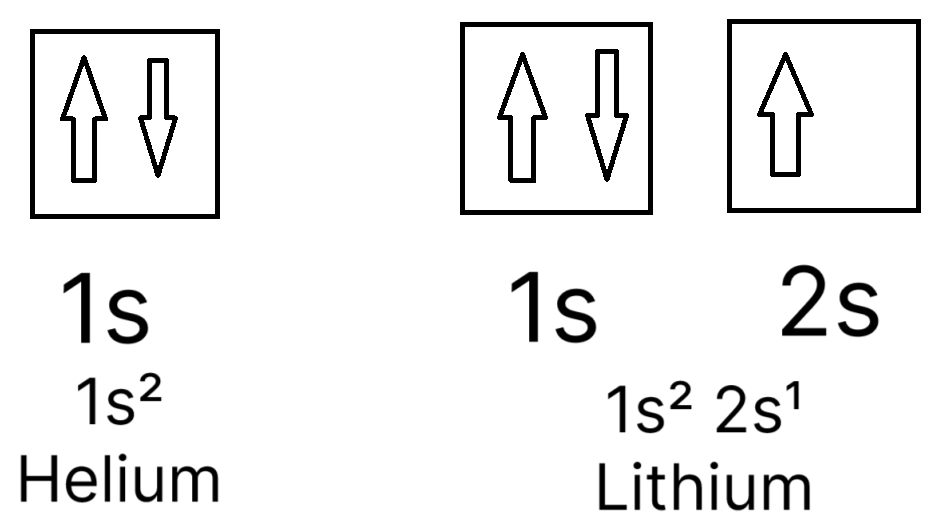
\includegraphics[width=0.5\linewidth]{chemistry/1.png}
    \caption{Orbital diagram and electron configuration of Helium and lithium}
    \label{fig:c1}
\end{figure}

We group orbitals from the same subshell by connecting the sides of the orbital boxes. \textbf{The Hund's rule} dictates how we should fill the atomic orbitals from the same subshell:
\begin{quote}
    Every orbital in a sublevel is singly occupied before any orbital is doubly occupied.
\end{quote}
In simple terms demonstrated by figure \ref{fig:c2}, you should fill all the orbitals in the same subshell with electrons of the same spin (\textit{in most cases}, up spin) before putting in the opposite spin.
\begin{figure}
    \centering
    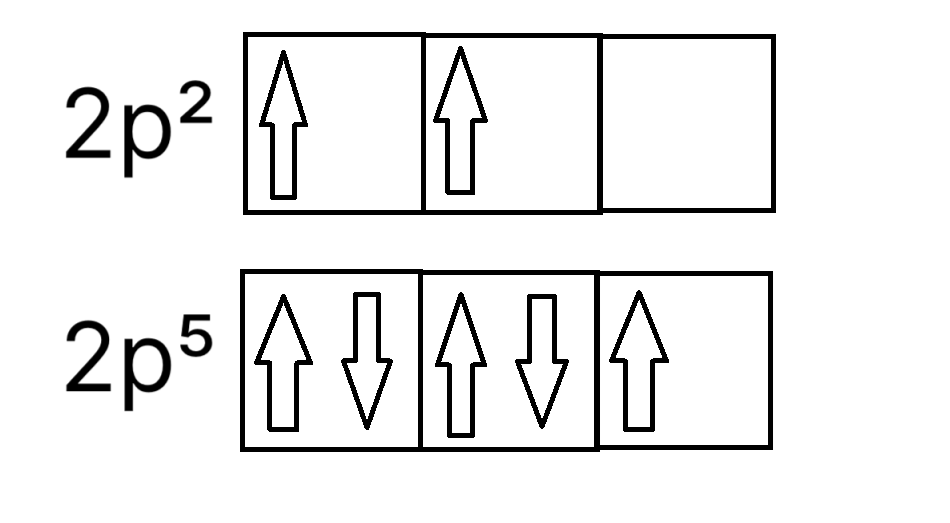
\includegraphics[width=0.5\linewidth]{chemistry/2.png}
    \caption{How electrons fill the orbits from the 2p subshell}
    \label{fig:c2}
\end{figure}

The number of orbitals per subshell is based on the third quantum number mentioned above: it is the number of possible values for $m_i$. The general formula for the number of atomic orbitals based on the second quantum number $l$ is:
\begin{equation} 1 + 2(l-1) \end{equation}
Multiply the result by 2 and you get the number of electrons a subshell can hold.

Another thing you need to keep in mind is the \textbf{Aufbau principle} ("Aufbau" in Germany translates to "build up", which suits its purpose of building electron configuration from the ground state up):
\begin{quote}
    When filling orbitals, the lowest energy orbitals available are always filled first.
\end{quote}
This principle is here to warn you of the fact that the subshell's energy level is not in order. Yes, the order \textit{inside a shell} follows the basic order based on $l$; however, an example would be the subshell 4s has a lower energy level compared to the 3d subshell. This is a reminder that $n$ is simply to show you the \textit{relative size} of the orbit (compared to a similarly shaped orbit) while $l$ is the shape — this is why the terminology "shell" is confusing in this case, as we tend to think they are orderly stacked but in fact, they are not (figure \ref{fig:c3}). Luckily, there is a trick to remember the energy level, presented in figure \ref{fig:c4}; the Aufbau principle starts to kick as we reach scandium, the first transition metal in the periodic table.
\begin{figure}
    \centering
    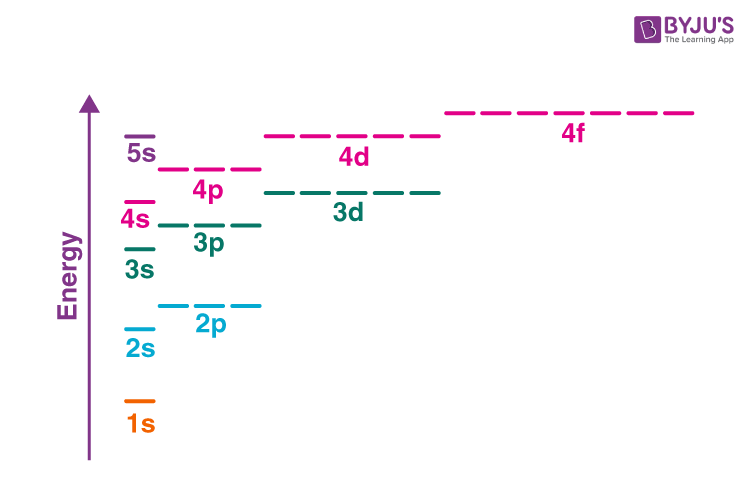
\includegraphics[width=0.75\linewidth]{chemistry/3.png}
    \caption{Energy diagram for each subshell, courtesy of BYJUS}
    \label{fig:c3}
\end{figure}
\begin{figure}
    \centering
    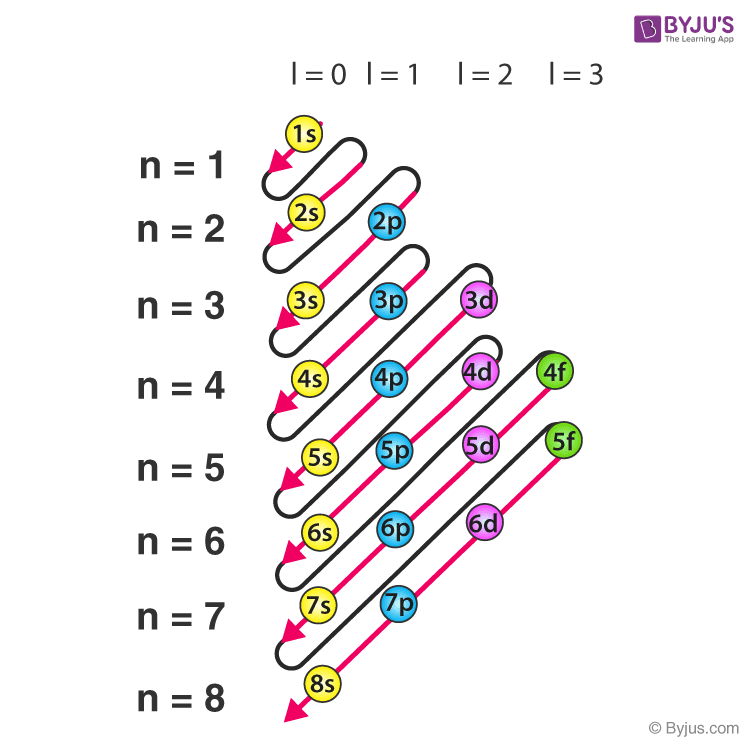
\includegraphics[height=0.7\linewidth]{chemistry/4.png}
    \caption{Aufbau principle's trick diagram, courtesy of BYJUS}
    \label{fig:c4}
\end{figure}

And just like any principle in chemistry, there are exceptions to the Aufbau principle. These exceptions are not very related to chemistry but it should not come as a surprise when encountering them.

To summarize this section, here is the list of things to think about when drawing an orbital diagram:
\begin{enumerate}
    \item Count how many electrons you need, then divide by 2 to have the number of boxes you will need to have
    \item Draw out the boxes with the correct shell subshell configuration. A simple tip to remember is 1, 3, 5, 7 for the s, p, d, and f subshell
    \item Fill the subshell: fill the entire subshell with up-spin electrons before filling it with down-spin (or vice versa for special cases)
    \item Stop when you already put down enough electrons, check if your element has a special case (usually question-dependent special cases)
\end{enumerate}

\section{Electron configuration}
Taking from figure \ref{fig:c1}, lithium's electron configuration has 3 electrons on two separate subshells — we write the number of electrons per subshell as a superscript after the subshell's notation. If we have $x$ as the number of electrons in a subshell, the general format for a subshell's electron configuration is:
\begin{equation}
    n\,l\,^x
\end{equation}
This makes the electron configuration for \ch{Li} which has 3 electrons as:
\begin{equation*}
    1s^2\;2s^1
\end{equation*}

Regarding the Aufbau principle, there are conflicting sources regarding whether you should sort according to the energy level or the shell's number order. This is up to you but consult your instructor for their preference. However, sorting by shell order is especially useful for writing the electron configuration of ions (which will be discussed later).

\textbf{The core notation} allows us to condense the electron configuration of elements based on the last noble gas before the element in the periodic table. This is because of the property where noble gas has a full valence shell. For example, sodium follows immediately after neon, so we can simplify to the core notation with warping \ch{Ne} in a square bracket:
\begin{equation*}
    1s^2 \; 2s^2 \; 2p^6 \; 3s^1
    \rightarrow
    [\text{Ne}] \; 3s^1
\end{equation*}

The valence shell (the outermost shell) is also how chemists name the blocks from the periodic table. From the example above, \ch{Na} is clearly from the s block, as its outermost subshell is s. Once again, keep in mind the Aufbau principle and the outermost shell is not necessarily the shell with the highest $n$ quantum number.

Recall that a cation has fewer electrons (positively charged) and an anion has more, which will in turn remove some electrons from the electron configuration. For \textit{only} cations, sort the neutral atom's electron configuration from the smallest to the largest, disregarding the Aufbau principle. After that, simply add or remove the electron according to your sorted order. Because of that, $\text{Sn}^{4+}$ should not be written as $\text{[Kr]} \; 5s^2 \; 4d^8$ but instead as:
\begin{equation*}
    \text{[Kr]} \; 4d^{10}
\end{equation*}

If an ion has the same electron configuration as another neutrally charged element, we call it \textbf{isoelectronic} with that element.